\documentclass[a4paper]{article}
\usepackage{cmap}
\usepackage{mathtext}
\usepackage{amssymb}
\usepackage{amsmath}
\usepackage[russian]{babel}
\usepackage{indentfirst}
\usepackage[pdftex]{graphicx}
\usepackage{multirow}
\usepackage{mathrsfs}
\usepackage{biblatex}
\usepackage{siunitx}
\usepackage[left=2cm,right=2cm,top=2cm,bottom=2cm]{geometry}
\usepackage{fancyhdr}
\bibliography{bib}
\pagestyle{fancy}
\newcommand{\const}{\mathrm{const}}
\newcommand{\rref}[1]{(\ref{#1})}
\newenvironment{comment}{}{}
\newcommand{\picref}[1]{рис. \ref{#1}}
\newcommand{\mbf}{\mathbf}
\newcommand{\Equip}[3]{
	
	{\bf #1:} $\Delta = \pm #2\; #3$}
\newcommand{\equip}[1]{
	
	{\bf #1}}
\newcommand{\labname}{Изучение голограммы} 	% название пиши здесь
\newcommand{\labnum}{4.3.5}		% номер вводи здесь
\fancyfoot{}
\fancyhead[RE, RO]{\thepage}
\fancyhead[LE, LO]{Лабораторная работа \labnum \space \labname}
\title{Лабораторная работа \labnum \space \labname} % Название работы здесь
\author{Иван Сладков}
\begin{document}
\maketitle
\thispagestyle{empty}
\section{Аннотация}
В данной работе проводится исследование голограмм точечного источника и объёмного предмета, а также изучение их свойств.

\section{Теоретические сведения}

Голография -- способ записи изображения, который позволяет по картине интенсивности восстановить полную информацию о волновом поле. Техника записи голограмм отображена на рис. \ref{fig:screenshot4}. Важным свойством голограммы является возможность восстановить по её малому участку информацию обо всём объекте. 

\begin{figure}[tbp]	
	\centering
	\begin{minipage}{0.49\linewidth}
		\centering
		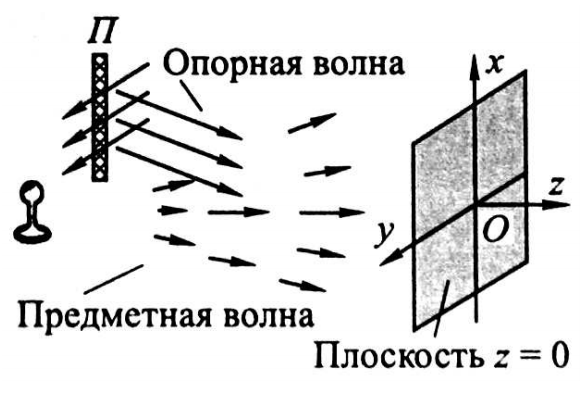
\includegraphics[width=0.8\linewidth]{Screenshot_4}
		\caption{Запись голограммы}
		\label{fig:screenshot4}
	\end{minipage}
	\begin{minipage}{0.49\linewidth}
		\centering
		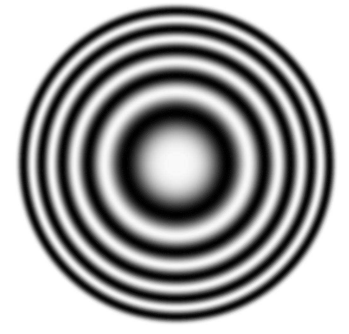
\includegraphics[width=0.8\linewidth]{Screenshot_1}
		\caption{Зонная решётка Габора}
		\label{fig:screenshot1}
	\end{minipage}
\end{figure}

Назовём волну, падающую на предмет, предметной; а волну, падающую сразу на плёнку -- опорной. Эти волны должны быть когерентны. Тогда:
\begin{equation*}\label{key}
	t \propto a^2+a_о^2+2 a a_o \cos (\varphi - \varphi_о),
\end{equation*}
то есть сохраняется информация о фазе волны.

В частности, для точечного источника, считая, что $ f_п = a e^{i k z}  $ и $ f_о \approx a e^{i k r} $, получаем голограмму  с функцией пропускания
\begin{equation*}\label{key}
	t(x, y) \propto \left| a+ a e^{i k r}\right|^2.
\end{equation*}

Для обратного процесса -- восстановления -- применяют плоскую нормально падающую волну. Считая $ f_- (x, y) \equiv 1, $ на выходе голограммы точечного источника получим:
\begin{equation*}\label{key}
	f_+ (x, y) = \left| a+ a e^{i k r}\right|^2 = 2 a^2 (1+\cos (k r)) = 2 a^2 + a^2 e^{i k r} +a^2 e^{- i k r}.
\end{equation*}
Отсюда видна структура полученной волны: суперпозиция плоской и двух сферических волн (соответствующих действительному и мнимому источникам).

Голограмма точечного источника имеет вид колец (рис. \ref{fig:screenshot1}) с радиусами
\begin{equation*}\label{key}
	\rho_m = \sqrt{m \lambda z_0},
\end{equation*}
где нечётному $ m $ соответствуют тёмные кольца.

Одним из свойств голограммы является её разрешающая способность, определяемая выражением:
\begin{equation*}\label{key}
	\Delta x \sim \frac{\lambda}{D} z_0,
\end{equation*}
где $ z_0 $ -- расстояние от источника до его голограммы, а $ D $ -- размер голограммы.

\section{Оборудование и инструментальные погрешности}

Схема экспериментальной установки отображена на рис. \ref{fig:screenshot2}.

\begin{figure}[tbp]
	\centering
	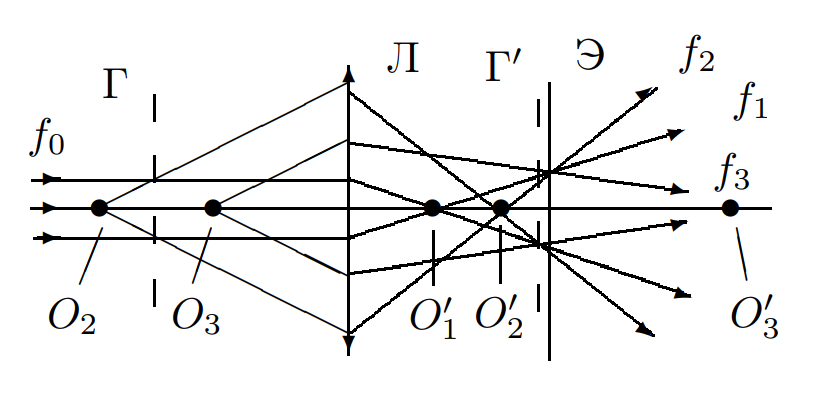
\includegraphics[width=0.8\linewidth]{Screenshot_2}
	\caption{Схема экспериментальной установки}
	\label{fig:screenshot2}
\end{figure}

В работе используются:
\equip{Лазер}: $ \lambda = 532 \; нм $
\equip{Голограммы}
\equip{Набор линз}: $ f = \left\{2\; мм, \; 43 \; мм, \; 78 \; мм,\; 200 \; мм\right\} $
\equip{Предметная шкала}
\equip{Экран}
\Equip{Линейка}{1}{мм}

\section{Результаты измерений и обработка данных}
\emph{Все измерения и расчёты в СИ.}

Расстояние между лазером и экраном: $ L = 98 \pm 0.5 \; см $

\subsection{Изучение голограммы точечного источника}

\paragraph{Настройка установки}

По формуле $ \lambda / D = \Delta x / L $, найдём $ D = 0.10 \; мм $. Кроме того, используя линзу $ f= 43\; мм $, по формуле $ b / a = D' / D $, получим $ D = 0.092 $, что близко к 1-му значению. В данных условиях 1-й метод даст большую точность, т. к. $ \Delta_\lambda\ll \Delta_f $.

\paragraph{Определение расстояния $ d $ от голограммы до точечного источника}

\label{источник}

Соберём микроскоп из линз $ f_1 = 43 \; мм $, $ f_2 = 78\; мм $. Зная цену деления шкалы, найдём $ \Gamma = 32 $. Построим график $ \rho^2(m) $ на рис. \ref{fig:screenshot3}.
\begin{figure}[tbp]
	\centering
	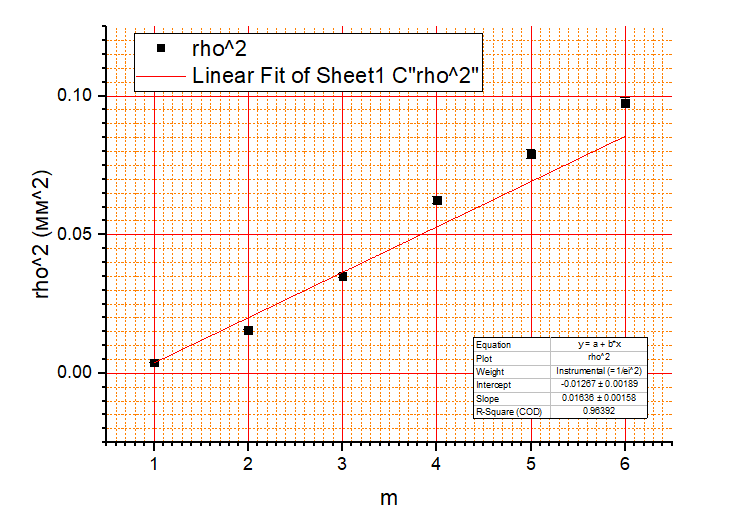
\includegraphics[width=0.8\linewidth]{Screenshot_5}
	\caption{График зависимости $\rho^2(m)$}
	\label{fig:screenshot3}
\end{figure}
Оттуда $ k =  0.016\pm 0.002 $ и $$ d = 30\pm 3 \; мм.$$
Величина ошибки получена из относительной случайной погрешности $ k $.

Получим изображения мнимого и действительного точечных источников:
\[ a_2 = 12 \pm 0.5 \; мм, \]
\[ a_3 = 82 \pm 2 \; мм. \]
Тогда расстояния от голограммы до источников $ d_i = a_i - f b_i /( b_i-f ) $, где $ b_i = L - a_i $:
\begin{equation*}\label{key}
	d_2 = 33\pm 1\; мм,
\end{equation*}
\begin{equation*}\label{key}
	d_3 = 37\pm 1\; мм.
\end{equation*}
Ошибки расчёта найдены по формуле инструментальных погрешностей.

\paragraph{Изучение фокусирующих свойств голограммы}

Определили, что правый пучок соответствует действительному источнику. 
В этом пучке $ D' = 1.5\pm 0.5 \; мм. $ Тогда по формуле $ b/f = D'/D $ найдём
\[ f = d = 38 \pm 12 \; мм. \]
Такая большая погрешность связана с несовершенством этого метода, т. к. сложно измерять расстояния около $ 1.5 \; мм $ в условиях засветки. 

Занесём результаты различных опытов в табл. \ref{tab:1}.

\begin{table}[h]
	\centering
	\begin{tabular}{|l|l|l|}
		\hline
		По диаметру колец & По расстоянию до изображения & По фокусирующим свойствам \\ \hline
		$15 \pm 1\; мм$   & $35\pm 2\; мм$               & $38\pm 12\; мм$           \\ \hline
	\end{tabular}
	\caption{Расстояния $d$ по результатам разных опытов}
	\label{tab:1}
\end{table}

\subsection{Изучение характеристик голограммы объёмного предмета}

Собрали расширитель пучка на основе двух линз. Диаметр пучка $ 2 r \approx 4 \; см $.

\paragraph{Изучение мнимого изображения}

Найдём мнимое изображение предмета в голограмме. Фото на рис. \ref{fig:ecwjolbkni}.
\begin{figure}[tbp]
	\centering
	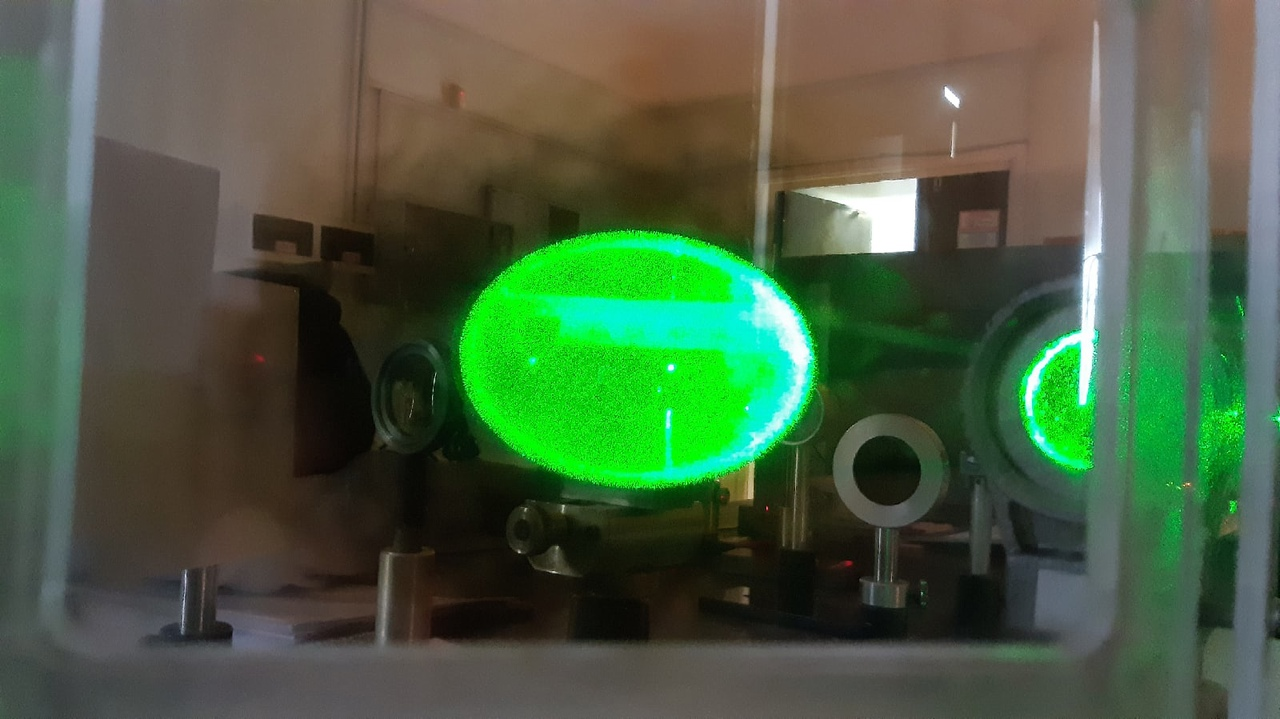
\includegraphics[width=0.8\linewidth]{ecwjo_LBknI}
	\caption{Мнимое изображение объёмного предмета}
	\label{fig:ecwjolbkni}
\end{figure}
Оценим угол поворота голограммы:
\[45^\circ \pm 5^\circ, \]
если вести отсчёт от положения перпендикулярного лучу.

Можно примерно (с погрешностью около $ 5^\circ $) оценить углы, под которыми край стержня совпадает с определёнными отметками линейки:
\[ \varphi = 90^\circ:\; l = 195.2, \]
\[\varphi = 110^\circ:\; l = 194.5. \]
Тогда расстояние от стержня до линейки
\[ h \approx 2.5\; см. \]
Эта величина очень приблизительная, так как край стержня видно плохо, и измерение углов <<на глаз>> даёт большую погрешность.

\paragraph{Изучение действительного изображения}

Удалось найти действительное изображение и даже сфокусировать его линзой на переносной экран. 

При повороте фотоэмульсией от лазера мнимое и действительное изображения меняются местами: теперь действительное наблюдается под углом $ 45^\circ $ справа против хода движения луча.

При перемещении короткофокусной линзы вдоль луча мнимое изображение не меняется. Масштаб действительного увеличивается при приближении линзы к голограмме.

\subsection{Оценка погрешностей}

Оценка погрешностей проводилась как и обычно. В общем, ни один из опытов по определению $ d $ не  обладает достаточной точностью, т. к. размеры измеряемых объектов часто небольшие, что ведёт к большим погрешностям. Наиболее перспективным является определение $ d  $ по радиусу колец, но в нашем случае недостаточно точек, т. к. следовало собрать микроскоп с б\'{о}льшим  увеличением.

\section{Вывод}

Изучили голограмму точечного источника и определили несколькими способами расстояние до записанного на неё точечного источника. Кроме того, изучили фокусирующие свойства голограмм точечного источника и исследовали некоторые особенности голограмм объёмного объекта. Интересная лабораторная.

\newpage

\begin{thebibliography}{9}
	\bibitem{Siv} Сивухин Д. В. \emph{Общий курс физики. Том 4 Оптика}, 2004
	\bibitem{kir} Кириченко Н. А. \emph{Принципы оптики}, 2014
	\bibitem{max} \emph{Лабораторный практикум по общей физике. В 3 томах. Том 2. Оптика: учебное пособие} под ред. А. В. Максимычева
\end{thebibliography}
\end{document}